%%%%%%%%%%%%%%%%%%%%%%%%%%%%%%%%%%%%%%%%%%%%%%%%%%%%%%%%%%%%%%%%%%%%%%%%%%
% SwitchOnBehaviorAndSwitchOffBehaviorOfPower
%%%%%%%%%%%%%%%%%%%%%%%%%%%%%%%%%%%%%%%%%%%%%%%%%%%%%%%%%%%%%%%%%%%%%%%%%%

\begin{solutionfigure}[ht]
    \centering
    \begin{subfigure}[t]{0.45\textwidth}
        \centering
        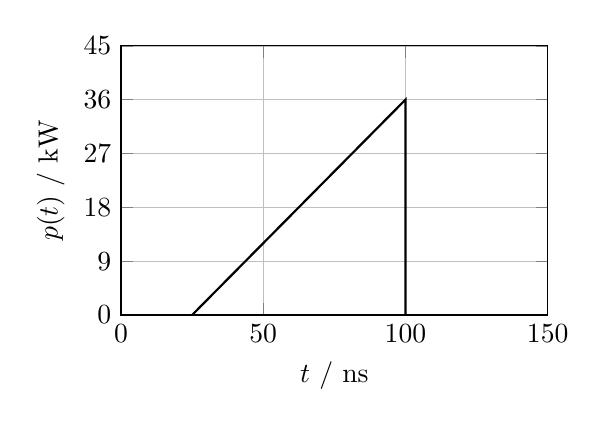
\begin{tikzpicture}
            \begin{axis}[
                width=7cm, height=5cm,
                grid=both,
                major grid style={line width=.2pt,draw=gray!50},
                minor grid style={line width=.1pt,draw=gray!20},
                xlabel={$t$ / ns},
                ylabel={$p(t)$ / kW},
                xmin=0, xmax=150,
                ymin=0, ymax=45,
                xtick={0, 50, 100, 150},
                ytick={0,9, 18, 27, 36, 45},
            ]
            % Einschaltverhalten graph
            \addplot[
                thick,
                mark=none,
                color=black,
            ] coordinates {
                (25,0) (100, 36) (100, 0)
            };
            \end{axis}
        \end{tikzpicture}
        \caption{Power values for the switch-on process.}
        \label{fig:Power values for the switch-on process}
    \end{subfigure}
    \hfill % Abstand zwischen den Subfiguren
    \begin{subfigure}[t]{0.45\textwidth}
        \centering
        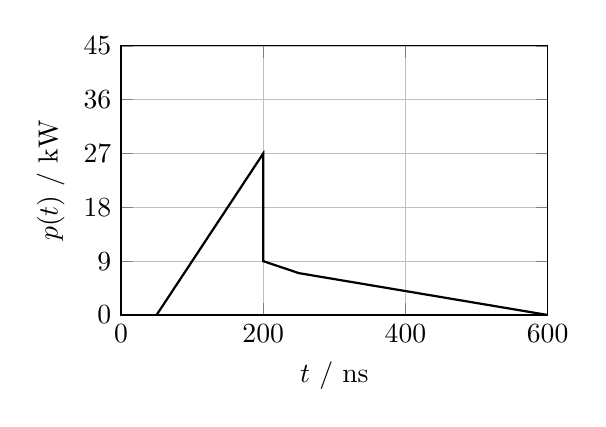
\begin{tikzpicture}
            \begin{axis}[
                width=7cm, height=5cm,
                grid=both,
                major grid style={line width=.2pt,draw=gray!50},
                minor grid style={line width=.1pt,draw=gray!20},
                xlabel={$t$ / ns},
                ylabel={$p(t)$ / kW},
                xmin=0, xmax=600,
                ymin=0, ymax=45,
                xtick={0,200, 400, 600},
                ytick={0,9, 18, 27,36, 45},
            ]
            % Ausschaltverhalten graph
            \addplot[
                thick,
                mark=none,
                color=black,
            ] coordinates {
                (50,0) (200, 27) (200, 9) (250, 7) (600,0)
            };
            \end{axis}
        \end{tikzpicture}
        \caption{Power values for the switch-off process.}
        \label{fig:Power values for the switch-off process}
    \end{subfigure}
    \caption{Switch-on behavior and switch-off behavior of $p(t)$}
\end{solutionfigure}

